\documentclass[a4paper]{article}
\usepackage[margin = 2.5cm]{geometry}
\usepackage[utf8]{inputenc}
\usepackage{amsmath,amssymb}
%\usepackage{subcaption, graphicx}
\usepackage[bottom]{footmisc}
\usepackage{graphicx}

\title{POPULATION GENETICS FOR SEQUENTIAL MONTE CARLO ALGORITHMS}
\author{\underline{S. Brown\textsuperscript{*}} \and P. Jenkins\textsuperscript{*$\dagger$} \and A. M. Johansen\textsuperscript{*$\ddagger$} \and J. Koskela\textsuperscript{*}}
\date{\small{\textsuperscript{*}Department of Statistics, University of Warwick, Coventry CV4 7AL\\
\textsuperscript{$\dagger$}Department of Computer Science, University of Warwick, Coventry CV4 7AL\\
\textsuperscript{$\ddagger$}The Alan Turing Institute, 96 Euston Rd, London NW1 2DB}}

\begin{document}
\maketitle

Sequential Monte Carlo (SMC) refers to a class of algorithms that use a simulated population of particles to approximate quantities of interest. 
Originally conceived for the simulation of molecular systems in physics, SMC methods are now used in a wide range of applications: forecasting weather, tracking military targets, interpreting medical test results, predicting financial crises, and much more.

The idea is to approximate a sequence of probability distributions arising in the system of interest, by simulating a population of particles whose evolution mimics the system's dynamics. There are three basic steps to the algorithm, which can be interpreted as the notions in population genetics of mutation, fitness and selection.

\vspace{5pt}

\begin{minipage}{0.45\textwidth}
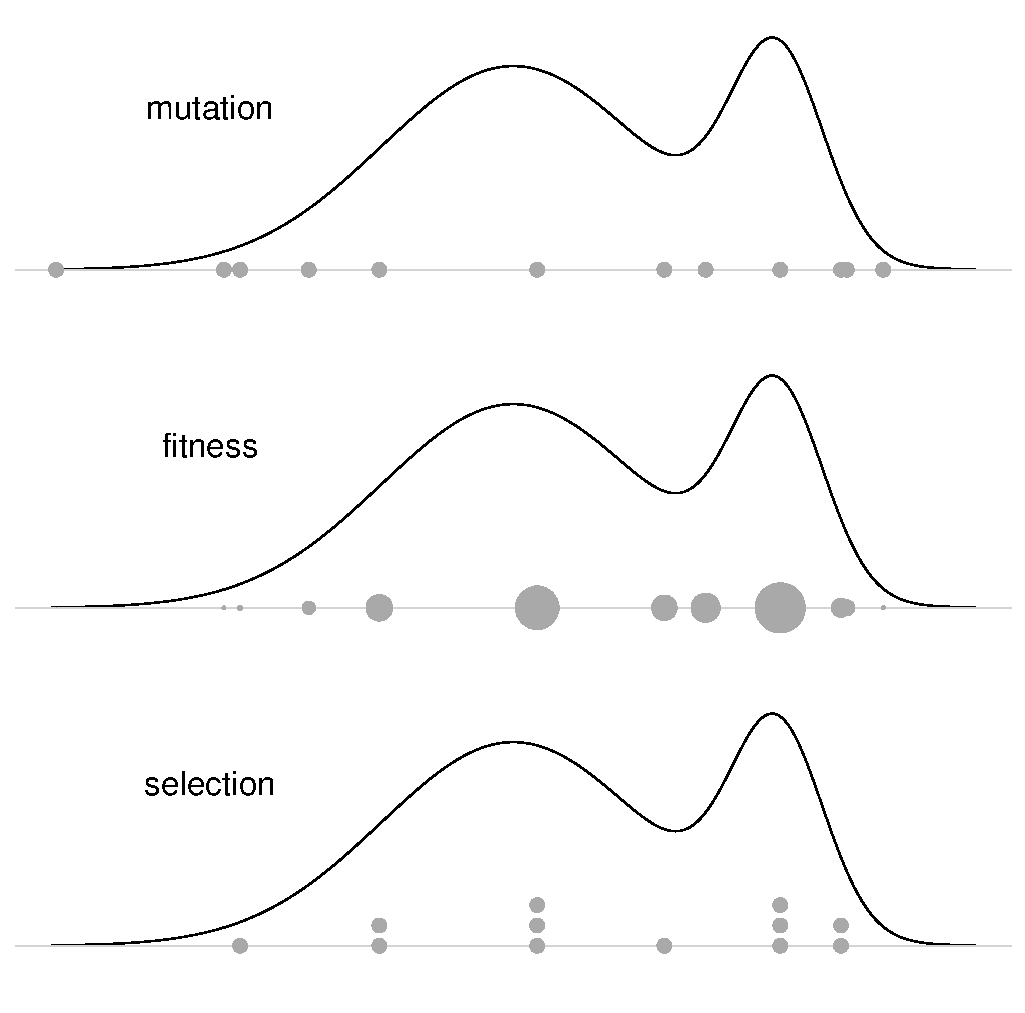
\includegraphics[width=0.8\textwidth]{smc_illustration.pdf}
\end{minipage}
\begin{minipage}{0.45\textwidth}
\begin{description}
\item[Mutation:] The positions of the particles are updated, according to the dynamics of the system of interest.
\item[Fitness:] A fitness value is calculated for each particle, according to how important the particle is in the approximation.
\item[Selection:] Particles reproduce in such a way that particles with high fitness are replicated many times, while particles with low fitness are killed off.
\end{description}
\end{minipage}

\vspace{5pt}

These three steps are repeated sequentially to produce a particle approximation to the distribution of interest at each time step.\\

The performance of the algorithm depends heavily on the selection mechanism used. My work focusses on analysing the role of selection, by describing the genealogies (family trees) arising in the population.
Genealogies arise naturally from selection, because each particle has a ``parent'' in the previous generation (the particle from which it was replicated). Tracing the parents of each particle, one can build up a genealogy of particles.

We make use of tools developed in the population genetics literature to apply to this artificial ``population''. 
For instance, it is known in population genetics that the genealogies of populations without selection converge to a process called Kingman's $n$-coalescent, as the population size grows to infinity.

SMC algorithms tend to have much stronger selection than the models typically used in population genetics. Nevertheless, we show that SMC algorithms using a variety of selection mechanisms also produce genealogies that converge to Kingman's $n$-coalescent as the population grows to infinity. To see this convergence, we have to rescale time by a random factor. The variation between the algorithms studied is seen through the different time scales on which the convergence takes place.\\

These results shed new light on the relative performance of different selection mechanisms in SMC, considering their effect on genealogies directly rather than considering the variance of the estimators, as has mostly been done in the past. Our results could help practitioners to choose better algorithms and parameters for their particular system, reducing the computational intensity of the SMC approximation, and thus allowing them to make better predictions for real world problems.


\thispagestyle{empty}
\end{document}